\documentclass[12pt]{article}
\usepackage[a4paper, total={7.5in, 10.5in}]{geometry}
\usepackage{array}
\usepackage{graphicx, subfig, wrapfig, fancyhdr, lastpage, multicol ,color,arydshln,makecell,chemfig}
\usepackage[most]{tcolorbox}
\newcommand\headerMe[2]{\noindent{}#1\hfill#2}
\usepackage[mathscr]{euscript}
\usepackage{tabularray}

\setlength{\columnseprule}{1pt}
\def\columnseprulecolor{\color{blue}}


\pagestyle{fancy}
\fancyhf{}

\cfoot{\vspace{-1cm} \em{Page \thepage \hspace{1pt} / 4}}


\newtcolorbox{Box2}[2][
enhanced, 
    breakable,
]{
                lower separated=false,
                colback=white,
colframe=white!20!black,fonttitle=\bfseries,
colbacktitle=white!30!gray,
coltitle=black,
enhanced,
attach boxed title to top left={yshift=-0.1in,xshift=0.15in},
title=#2,#1
}
%    \vspace{.2cm}



\begin{document}

\headerMe{Royaume du Maroc}{année scolaire \emph{2023-2024}}\\
\headerMe{Ministère de l'Éducation nationale, }{  }\\
\headerMe{du Préscolaire et des Sports}{Établissement : \emph{Lycée SKHOR qualifiant}}\\
\vspace{-1cm}
\begin{center}
%Devoir Surveillé  N°1 \\
  \textbf{Soutien}\\
    2ème année baccalauréat Sciences Physiques\\
%Durée 2h00
%    \vspace{.2cm}
\hrulefill
  \Large{--Chimie--}
\hrulefill\\

    \emph{Les  parties sont indépendantes}
    %\emph{Les deux parties sont indépendantes}

    \vspace{-.2cm}
\end{center}
%end Headerss------------------------
%__________________Chimie ______________________-
%%%%%%%+_+_+_+_+_+_+_+_+_Partie1
\begin{Box2}{SN2020:Etude de quelques réactions de l’éthanoate de sodium}
 \emph{L’éthanoate de sodium est un solide blanc de formule $CH_3COONa$ . On le trouve dans le
commerce sous forme de pochettes vendues comme sources de chaleur portatives. Lors de sa
dissolution dans l’eau, on obtient une solution aqueuse d’éthanoate de sodium $(Na^+_{(aq)} + CH_3COO^-_{(aq)})$} 

Cet exercice se propose d’étudier :
- une solution aqueuse d’éthanoate de sodium.
- la réaction des ions éthanoate avec l’acide méthanoïque HCOOH.

\textbf{Données :}
\begin{itemize}
  \item Le produit ionique de l’eau: $K_e = 10.^{-14}$ à 25°C.
\end{itemize}

  \textbf{I-Etude d’une solution aqueuse d’éthanoate de sodium}
  On prépare une solution aqueuse S d’éthanoate de sodium de concentration $C = 10^{-3}mol/L$
La mesure du pH de la solution S donne : $pH = 7,9$.

  \begin{enumerate}
    \item Ecrire l’équation de la réaction des ions éthanoate $CH_3COO^-$ avec l'eau.
    \item Calculer la concentration effective des ions hydroxyde $HO^-_{(aq)}$ dans la solution S.
    \item Calculer le taux d’avancement final $\tau$ de la réaction. Que peut-on déduire ?
    \item Trouver, à l’équilibre, l’expression du quotient de la réaction
$Q_{r,eq}$ associé à cette réaction en fonction de $C$ et $\tau$ Calculer sa valeur.
\item Vérifier que le $pK_A$ du couple $CH_3COOH/CH_3COO^-$ est $pK_{A1} = 4,8$.

\end{enumerate}
  \textbf{II-Réaction entre les ions éthanoate et l’acide méthanoïque}
  On prépare, à un instant de date t = 0, le mélange suivant constitué:
  \begin{itemize}
        \item d'un volume $V_1 = 100mL$ d’une solution aqueuse d’acide méthanoïque $HCOOH_{(aq)}$ de concentration $C_1=0,1mol/L$.
        
        \item d'un volume $V_2 = 100mL$ d’une solution aqueuse d’éthanoate de sodium $Na^+_{(aq)} + CH_3COO^-_{(aq)}$ de concentration $C_2=0,1mol/L$.
        \item d'un volume $V_3 = 100mL$ d’une solution aqueuse d’acide éthanoïque $CH_3COOH_{(aq)}$ de concentration $C_3 = 0,1 mol/L$

        \item d'un volume $V_4 = 100mL$ d’une solution aqueuse de méthanoate de sodium $Na^+_{(aq)} + HCOO^-_{(aq)}$ de concentration $C_4=0,1mol/L$.

          \begin{enumerate}
            \item  Ecrire l’équation de la réaction entre l’acide $HCOOH$ et la base $CH_3COO^-$.
            \item Trouver l’expression de la constante d’équilibre K associée à cette réaction en fonction de la constante d’acidité $K_{A1}$ du couple $CH_3COOH /CH_3COO^-$  et la constante d'acidité $K_{A2}$ du couple $HCOOH / HCOO^-$.Calculer sa valeur sachant que $pK_{A2} = 3,8$.
            \item Calculer, à l’instant t = 0, le quotient de réaction $Q_{r,i}$ associé à cette réaction.
            \item En déduire le sens d’évolution spontanée de cette réaction.
            \item Sachant que l’avancement à l’équilibre de la réaction est :$x_{eq} = 5,39.10^{-3}mol$, déterminer la
valeur du pH du mélange.

          \end{enumerate}
  \end{itemize}
\end{Box2}

\begin{Box2}{SR2023:Dosage d’une solution aqueuse de triméthylamine}
  \emph{La triméthylamine, de formule brute $(CH_3)_3N$, est une molécule présente dans quelques aliments. Elle a
une odeur caractéristique de poisson pourri. Elle est également associée à une maladie génétique appelée
  syndrome de l’odeur de poisson pourri. La triméthylamine est éliminée par les urines, les sueurs ...}
  
On admet qu’un patient est atteint de syndrome de l’odeur de poisson pourri si la concentration en
triméthylamine dans son urine est supérieure à $2,2.10^{-10} mol/L$
  \textbf{Données : }
\begin{itemize}
  \item Toutes les mesures sont effectuées à $25^{\circ}C$
  \item Couple acide-base lié à la triméthylamine:  ${(CH_3)_3NH^+}_{(aq)}/ {(CH_3)_3N}_{(aq)}$.
 
\end{itemize}

Pour doser une solution $S_0$ d’urine d’un patient dont la concentration en triméthylamine est C0, on la dilue
10 fois pour obtenir une solution $S_B$ de concentration $C_B$.

On prend le volume $V_B = 20mL$ de la solution $S_B$ auquel on ajoute progressivement un volume $V_A$ d’une solution aqueuse $S_A$ d’acide chlorhydrique $({H_3O^+}_{(aq)} + {Cl^-}_{(aq)})$ de concentration $C_A = 4.10^{-2}mol/L$. 
  
  On suppose que l’acide chlorhydrique réagit seulement avec la triméthylamine. La courbe représentant la variation du pH du mélange réactionnel en fonction du volume $V_A$ de la solution acide $S_A$ ajoutée présente deux points remarquables :

\begin{itemize}
  \item le point Q de coordonnées $V_A = 10mL$ et $pH=9,9$.
  \item le point d'équivalence E de coordonnées $V_{AE} = 20mL$ , $pH_E = 5,8$
\end{itemize}


  \begin{enumerate}
    \item Définir une base selon Bronsted. (0,5pt)
    \item Ecrire l’équation modélisant la réaction qui a lieu lors du dosage. (0,5pt)
    \item Déterminer la valeur de $C_B$. (0,5pt)
    \item Déduire que le patient est atteint du syndrome de l’odeur de poisson pourri. (0,5pt)
    \item Justifier la nature acide $pH_E < 7$ du mélange réactionnel à l’équivalence.
    \item Parmi les indicateurs colorés cités dans le tableau ci-dessous, indiquer en justifiant celui qui convient le
mieux pour ce dosage. (0,5pt)
\begin{center}
\begin{tabular}{ |c|c|c|c| } 
 \hline
  Indicateur coloré & Hélianthine & Rouge de méthyle & phénolphtaléine \\\hline 
  Zone de virage & 3,1-4,4 & 4,2-6,2 & 8,2-10,0 \\ 
 \hline
\end{tabular}
\end{center}
\item En se basant sur le tableau d’avancement de la réaction de dosage, trouver la valeur du rapport 
  $$\frac{[{(CH_3)_3NH^+}_{(aq)}]}{[{(CH_3)_3N}_{(aq)}]}$$ pour $V_A = 10mL$
\item 8- Déduire que la valeur du $pK_A$ du couple ${(CH_3)_3NH^+}_{(aq)} / {(CH_3)_3N}_{(aq)} $ est $pK_A = 9,9$
\end{enumerate}

\end{Box2}
\vspace{2cm}
\begin{center}
 \hrulefill
  \Large{--Mécanique--}
\hrulefill\\

\end{center}
%\vspace{-1.0cm}

 \begin{Box2}{SR2023:Etude du mouvement d’un ballon dans un champ de pesanteur uniforme}

   Lors d’un service, un joueur de volley-ball, se trouvant à une distance D du
filet, frappe le ballon à une hauteur h du sol et lui communique une vitesse $\vec{V_0}$
faisant un angle $\alpha$ par rapport à l’horizontale.

   A cet instant choisi comme origine des dates $t_0 = 0$
, le centre d’inertie G du ballon est au point A (figure 1).
  
   \begin{center}
%	  \vspace{-2cm}
	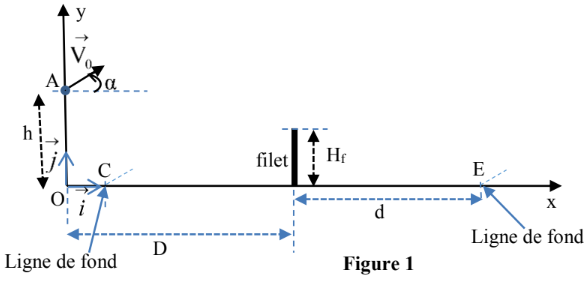
\includegraphics[width=0.6\textwidth]{./img/chute_libreSx.png}
  \end{center}
   \textbf{Données}

 \begin{itemize}
   \item $V_0 = 16 m/s$ ; $\alpha = 18^{\circ}$ ; $D=11m$ ; $h = OA= 3m$
   \item Hauteur du filet : $H_f = 2,4m$
   \item Distance entre le filet et la ligne de fond : $d =9m$
   \item Intensité de la pesanteur $g = 10 m.s^{-2}$
 \end{itemize}
   On étudie le mouvement du centre d’inertie G du ballon dans le repère $(O,\vec{i} , \vec{j} )$lié à un référentiel terrestre
considéré galiléen. L’origine O est situé au niveau du sol (figure 1).

On considère que le ballon est en chute libre.

\begin{enumerate}
  \item En appliquant la deuxième loi de Newton, établir les équations horaires x(t) et y(t) du mouvement de G. (1pt)
  \item Déduire que l’équation de la trajectoire du mouvement de G s’écrit: $$y = - \frac{1}{2}. \frac{g}{(V_0.cos\alpha)^2}.x^2 + (tan\alpha).x + h$$
  \item Montrer que le ballon passe au-dessus du filet (on néglige le rayon du ballon devant Hf). (0,75pt)
  \item Le ballon atteindra le sol à l’instant $t_s=1,41s$
    Le ballon tombe-t-il entre le filet et la ligne du fond du camp adverse? Justifier. (0,75pt)
\end{enumerate}


 \end{Box2}

\vspace{2cm}

\begin{Box2}{SR2020:Etude du mouvement d’un solide sur un plan horizontal }

  \begin{wrapfigure}{r}{0.5\textwidth}
    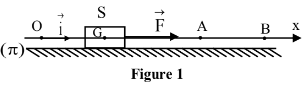
\includegraphics[width=0.5\textwidth]{./img/planpi.png} 
  \end{wrapfigure}
  
  \emph{Cet exercice se propose d’étudier le mouvement d’un solide sur un plan horizontal.
Un solide S de masse m et de centre d’inertie G . glisse sans frottement sur un plan horizontal $\pi$.}
Le solide S est en mouvement sur la partie OA
du plan sous l’action d’une force motrice
horizontale constante (figure 1).

\begin{itemize}
  \item m=2Kg;
  \item OA=2,25m;
\end{itemize}

  \begin{wrapfigure}[5]{r}{0.34\textwidth}
    \vspace{-4cm}
    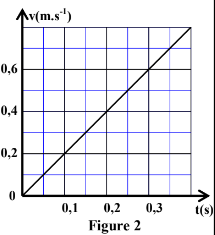
\includegraphics[width=0.34\textwidth]{./img/vitesse_plan.png} 
  \end{wrapfigure}
  
On étudie le mouvement de G dans un repère
$(O, \vec{i} )$
lié à un référentiel terrestre supposé galiléen

et on repère la position de G à chaque instant par son abscisse x(t).
A l’instant t = 0, le centre G et l’origine O sont confondus.
Un système d’acquisition informatisé permet de tracer la courbe
représentant l’évolution de la vitesse de G sur la partie OA(figure 2).

\begin{enumerate}
  \item En appliquant la deuxième loi de Newton, montrer que
    l’équation différentielle vérifiée par l’abscisse x(t) est :$\frac{d^2x}{dt^2} = \frac{F}{m}$
  \item En exploitant le graphe de la figure 2, vérifier que l’accélération
    du mouvement de G est $a_G = 2 m.s^{-2}$
  \item En déduire l’intensité de $\vec{F}$
  \item Montrer que l’équation horaire du mouvement de G sur la partie OA, dans le système
international d’unités, s’écrit : $x = t^2$.
\item Lors du passage de G par le point A, on élimine la force . le solide poursuit alors son
mouvement sur la portion AB.
\begin{enumerate}
  \item Montrer que le mouvement de G sur la partie AB est rectiligne uniforme.
  \item Trouver alors la vitesse $V$ de G sur la partie AB.

\end{enumerate}
\end{enumerate}


\end{Box2}



\end{document}
